%% LaTeX2e Template by Stephen Iota (https://stepheniota.com/)
%% last updated: May 2019
\documentclass{article}
\usepackage[a4paper,margin=2cm]{geometry}
\usepackage[utf8]{inputenc}
%\usepackage[noadjust]{cite}
\usepackage{lipsum}
\usepackage{amsmath,amssymb,amsfonts,physics}
\usepackage{mathtools} % for boxed answers in align environments
\usepackage{graphicx} % \includegraphics{ }
\usepackage[shortlabels]{enumitem} % change labels in enum/item environments
\usepackage[dvipsnames]{xcolor} % colored links=
%\usepackage[big]{titlesec} % [small,medium,big] << controls size of *section text
%\usepackage{fancyhdr} %http://tug.ctan.org/tex-archive/macros/latex/contrib/fancyhdr/fancyhdr.pdf
\usepackage[
	colorlinks=true,
	citecolor=green!50!black,
	linkcolor=Red,
	urlcolor=green!50!black,
	hypertexnames=false]{hyperref}
 %%%%%%%%%%%%%%%%%%
 %% New Commands %%
 %%%%%%%%%%%%%%%%%%
\newcommand{\email}[1]{\texttt{\href{mailto:#1}{#1}}}
\newcommand{\HH}[0]{\ensuremath{\mathcal{H}}}
%\newcommand{\ave}[1]{$\langle #1 \rangle$}
\renewcommand{\d}[1]{\ensuremath{\operatorname{d}\!{#1}}}

\newenvironment{question}[0]{
\vspace{2mm}
\noindent
\itshape
}

\newenvironment{solution}[0]{
\vspace{2mm}
\noindent
\textbf{Solution:}
}

%%%%%%%%%%%%%%%%%%
%% Front Matter %%
%%%%%%%%%%%%%%%%%%
%\pagenumbering{gobble} % no page numbers
\graphicspath{{figures/}} % set directory for figures
%\setcounter{section}{-1} % start with section 0
\numberwithin{equation}{section}
%%%%%%%%%%%%%
%%% Title %%%
%%%%%%%%%%%%%
\begin{document}

\begin{center}
{\Large \textsc{Statistical Mechanics}: \textbf{Problem Set 3}}
\end{center}
\vspace{.5mm}

%%%%%%%%%%
%% INFO %%
%%%%%%%%%%

\begin{tabular}{rl}
\textsc{Name}:			&		Stephen Iota (\email{siota001@ucr.edu})
\\
\textsc{Course}:		&		Physics 133 (Spring 2019), Prof.~Kuhlman
\\
\textsc{Date}:			&		\today
\end{tabular}
\vspace{2mm}

%%%%%%%%%%%%%%
%% PROBLEMS %%
%%%%%%%%%%%%%%

\noindent
Sethna problems 3.6, 3.8, 5.1 and 5.5.  All final answers are \boxed{\text{boxed}}.

%%%%%%%%%%%%%%%%%%%%%%%%%%%%%%%%%%
%% CONNECTING TWO MACRO SYSTEMS %%
%%%%%%%%%%%%%%%%%%%%%%%%%%%%%%%%%%
\section{Connecting two macroscopic systems}
An isolated system with energy $E$ is composed of two macroscopic subsystems, each of fixed volume $V$ and number of particles $N$. The subsystems are weakly couples, so the sum of their energies is $E_1 + E_2 = E$. The volume of the energy surface of a system with the Hamiltonian $\mathcal{H}$ is given by
\begin{align}
\Omega(E) &= \int \frac{\d{\mathbb{P}}\d{\mathbb{Q}}}{h^{3N}} \ \delta(E - \mathcal{H}(\mathbb{P},\mathbb{Q}))
\\
					&= \int \frac{\d{\mathbb{P}_1}\d{\mathbb{Q}_1}}{h^{3N_1}}
					\frac{\d{\mathbb{P}_2}\d{\mathbb{Q}_2}}{h^{3N_2}} \
					\delta(E - (\mathcal{H}_1(\mathbb{P}_1,\mathbb{Q}_1)+\mathcal{H}_2(\mathbb{P}_2,\mathbb{Q}_2)).
					\label{omega}
\end{align}

\begin{question}
Derive the formula $\Omega(E) = \int \d{E_1} \ \Omega_1(E_1) \Omega_2(E-E_1),$ for the volume of the energy surface of the energy surface of the whole system using Dirac $\delta$-functions.
\end{question}

\begin{solution}
Beginning with the definition for the volume of the energy surface of a system with Hamiltonian $\HH$ [\ref{omega}], we insert the identity $ \int \d{E_1} \ \delta(E_1 - \HH_1) = 1$. Grouping the integrals together, we notice the definition for $\Omega(E_1)$ where the delta-function picks out $E_1 = \HH_1$. We then do the same for the next integral, where the delta-function now picks out $E - E_1 = \HH_2$.
\begin{align}
\Omega(E) &= \iiint \d{E_1} \ \delta(E_1 - \HH_1) \
				 \frac{\d{\mathbb{P}_1}\d{\mathbb{Q}_1}}{h^{3N_1}}
				 \frac{\d{\mathbb{P}_2}\d{\mathbb{Q}_2}}{h^{3N_2}} \
			 	 \delta(E - (\HH_1+\HH_2))
				 \\
			 &= \int \d{E_1}
			    \int \frac{\d{\mathbb{P}_2}\d{\mathbb{Q}_2}}{h^{3N_2}}\ \delta(E - (\HH_1+\HH_2)
				 \int \frac{\d{\mathbb{P}_1}\d{\mathbb{Q}_1}}{h^{3N_1}}\  \delta(E_1 - \HH_1)
				 \\
			 &= \int \d{E_1} \ \Omega(E_1)
			    \int \frac{\d{\mathbb{P}_2}\d{\mathbb{Q}_2}}{h^{3N_2}}\delta(E - E_1 - \HH_2)
				 \\
\Aboxed{
\Omega(E) &= \int \d{E_1} \ \Omega(E_1) \ \Omega(E - E_1)
}
\end{align}
\end{solution}


\newpage
%%%%%%%%%%%%%%%%%%%%%%%%%%%%%%%%%
%% MICROCANONICAL ENERGY FLUCT %%
%%%%%%%%%%%%%%%%%%%%%%%%%%%%%%%%%
\section{Microcanonical energy fluctuations}
For two subsystems with energy $E_1$ and $E_2 = E - E_1$ the probability density of $E_1$ is a Gaussian with variance
\begin{align}
\sigma_{E_1}^{2} &= -k_B/(\pdv[2]{S_1}{E_1} + \pdv[2]{S_{2}}{E_2}). \label{variance}
\end{align}

\begin{question}
\textnormal{\textbf{(a)}}
Show that
				\begin{align}
				\frac{1}{k_B} \pdv[2]{S}{E} &= - \frac{1}{k_BT} \frac{1}{Nc_vT}
				\label{fluctuation}
				\end{align}
				where $c_v$ is the inverse of the total specific heat at constant volume.
\end{question}

\begin{solution}
The equilibrium entropy is $ S = k_B \log(\Omega(E)) $ where temperature is defined as $ 1/T \equiv \partial S / \partial E.$ Using some sleight of hand Leibniz notation\footnote{Mathematicians beware!}:
\begin{align}
\frac{1}{k_B}\pdv[2]{S}{E} &= \frac{1}{k_B}\pdv{E}\pdv{S}{E}
\\
&= \frac{1}{k_B}\pdv{E} \frac{1}{\Omega}\pdv{\Omega}{E}
\\
&= \frac{1}{k_B}\pdv{E} \frac{1}{T}
= \frac{1}{k_B} \pdv{E} \pdv{T}{T} \frac{1}{T}
\\
&= \frac{1}{k_B} \pdv{T}{E} \pdv{\frac{1}{T}}{T}
= -\frac{1}{k_B} \frac{1}{Nc_v} \frac{1}{T^2}
\\
\Aboxed{\frac{1}{k_B}\pdv[2]{S}{E} &= -\frac{1}{k_B T} \frac{1}{Nc_vT}}
\end{align}
where we made use of the specific heat $Nc_v \equiv \partial E / \partial T$.
\end{solution}



\begin{question}
\textnormal{\textbf{(b)}}
If $c_{v1}$ and $c_{v2}$ are the specific heats per particle for two subsystems of $N$ particles each, show using eqns [\ref{variance}] and [\ref{fluctuation}] that
				\begin{align}
				\frac{1}{c_{v1}} + \frac{1}{c_{v2}} = \frac{Nk_BT^2}{\sigma_{E_1}^2}.
				\end{align}
\end{question}
\begin{solution}
This one is pure massaging equations, specifically [\ref{variance}] and [\ref{fluctuation}].
\begin{align}
\sigma_{E_1}^{2} &= -k_B/\bigg(\pdv[2]{S_1}{E_1} + \pdv[2]{S_{2}}{E_2}\bigg)
\\
\pdv[2]{S_1}{E_1} + \pdv[2]{S_{2}}{E_2} &= -k_B/\sigma_{E_1}^{2}
\end{align}
We substitute in the specific heat $Nc_v$ for each subsystem.
\begin{align}
-\frac{1}{NT^2}\bigg( \frac{1}{c_{v1}} + \frac{1}{c_{v2}} \bigg) &= -\frac{k_B}{\sigma_{E_1}^{2}}
\\
\Aboxed{\frac{1}{c_{v1}} + \frac{1}{c_{v2}} &= \frac{Nk_BT^2}{\sigma_{E_1}^{2}}} \label{sum}
\end{align}

\end{solution}




\begin{question}
\textnormal{\textbf{(c)}}
Using the equipartition theorem, write the temperature in terms of $K$. Show that $c_v^{(1)} = 3k_B/2$ for the momentum degrees of freedom. In terms of $K$ and $\sigma_K$, solve for the total specific heat of the molecular dynamics simulation.
\end{question}

\vspace{2mm}
\noindent
\textbf{Solution:}\\
\emph{Temperature in terms of $K$.}
The kinetic energy of a particle moving in a direction $i$ is given by $p_i^2/2m$. The average kinetic energy of a particle depends on the temperature of its system $K = 1/2 k_B T$. A particle has three translational degrees of freedom, each of which contribute equally---on average---to the average to the particle's kinetic energy (equipartition theorem). Thus for a gas of $N$ atoms, its total average kinetic energy is
\begin{align}
K &= \frac{3}{2} N k_B T.\label{kinetic}
\end{align}
This allows us to write the temperature as a function of energy as $\boxed{T(K) = \frac{2}{3}\frac{E}{Nk_B}}$.

\vspace{2mm}
\noindent
\emph{Momentum degrees of freedom.}
Remebering the definition of specific heat, we rewrite energy in terms of temperature to show $c_v^{(1)} = 3k_B/2$ for the momentum degrees of freedom.
\begin{gather}
Nc_{v1} = \pdv{E}{T_1} = \pdv{T_1} \bigg( \frac{3}{2} N k_b T_1 \bigg)
\\
\boxed{c_{v1} = 3/2 k_B}\label{specific_heat}
\end{gather}


\vspace{2mm}
\noindent
\emph{Total specific heat.}
First note that $\sigma_K = \sigma_{E}$.
Let $K = \langle E_1 \rangle$. Since the kinetic energy does not depend on the spacial configuration $\mathbb{Q}$ and potential energy does not depend on momentum configuration $\mathbb{P}$, we can treat our system as two uncoupled-subsystems, where $c_{v1}$ is the kinetic contribution to specific heat and $c_{v2}$ is the configuration contribution. Plug in [\ref{kinetic}] and [\ref{specific_heat}] to [\ref{sum}].
\begin{gather}
\frac{1}{c_{v2}} = \frac{Nk_BT^2}{\sigma^2_{E_1}} - \frac{2}{3}k_BT
\\
\frac{1}{c_{v2}} = \frac{1}{N k_B \sigma^2_{E_1}} \bigg(4K^2 - 6Nk_B^2 \sigma^2_{E_1}  \bigg)
\\
c_{v2} = \frac{N k_B \sigma^2_{E_1}}{4K^2 - 6Nk_B^2 \sigma^2_{E_1}}
c_{v2} = \frac{(k_B N \sigma^2_K)}{4K^2 - 6N\sigma^2_K}
\end{gather}
Then we find that $c_{v1} + c_{v2}$ is
\begin{align}
c_v &= c_{v1} + c_{v2}
\\
&= \frac{(k_B N \sigma^2_K)}{4K^2 - 6N\sigma^2_K} + \frac{3}{2}k_B
\\
\Aboxed{
c_v &= k_B \frac{K^2}{\frac{2}{3}K^2 - N\sigma_K^2}}
\end{align}


\newpage
%%%%%%%%%%%%%%%%%%%%%%%%%%%%%%%%%
%% MICROCANONICAL ENERGY FLUCT %%
%%%%%%%%%%%%%%%%%%%%%%%%%%%%%%%%%
\section{Life and the heat death of the universe}

\emph{Living beings intercept entropy flows}; they use low-entropy sources of energy and emit high-entropy forms of the same energy. Freeman Dyson presumed that an intelligent being generates a fixed entropy $\Delta S$ per thought. Let's investigate how living beings might evolve to cope with the cooling and dimming we expect during the heat death of the Universe.\\
Assume that a being draws heat Q from a hot reservoir at $T_1$ and radiates it away to a cold reservoir at $T_2$.

\begin{question}
\textnormal{\textbf{(a)}}
\textbf{\emph{Energy needed per thought.}}
What is the minimum energy $Q$ needed per thought, in terms of $\Delta S$ and $T_2$?
\end{question}

\begin{solution}
The change in entropy $\Delta S$ is given by
\begin{align}
	\Delta S &= \frac{Q_2}{T_2} - \frac{Q_1}{T_1}\label{entropy}.
\end{align}
If our heat bath $T_1$ is very hot, we can ignore the last tern in [\ref{entropy}] and we're left with
\begin{align}
	\Delta S &= \frac{Q_2}{T_2}
\end{align}
Thus, the minimum energy $Q$ needed per thought is given by
\begin{align}
\Aboxed{	Q &= T_2\Delta S.}\label{Q}
\end{align}
\end{solution}

\begin{question}
\textnormal{\textbf{(b)}}
\textbf{\emph{Time needed per thought to radiate energy.}}
Write an expression for the maximum rate of thoughts per unit time $\dv*{H}{t}$ (the inverse of the time $\Delta t$ per thought), in terms of $\Delta S$, $C$, and $T_2$.
\end{question}

\begin{solution}
Let $H$ be number of thoughts. Dyson shows that power radiated by our intelligent-being-as-entropy-producer is about
$P = C T^3_2$.
It follows that the energy radiated for a thought of time $\tau$ is
$E = C T^3_2 \tau$.

This energy is simply energy $Q$, the heat energy taken from the hot bath $T_1$.
The time-per-thought $\tau$ is
\begin{align}
\tau &= \frac{\Delta S}{C T^2_2}\label{time}
\end{align}
The time needed per thought $\dv*{H}{t}$ is [\ref{time}]'s reciprocal.
\begin{align}
\Aboxed{ \dv{H}{t} &= \frac{C T^2_2}{\Delta S}}
\end{align}
\end{solution}




\begin{question}
\textnormal{\textbf{(c)}}
\textbf{\emph{Number of thoughts for an ecologically efficient being.}}
\emph{Our Universe is expanding ($R \sim t$); the microwave background radiation has a characteristic temperature $\Theta (t) \sim R^{-1}$ which is getting lower as the Universe expands due to the Doppler effect.}
How many thoughts $H$ can an ecologically efficient being have between now and time infinity, in terms of $\Delta S$, $C$, $A$, and the current time $t_0$?
\end{question}

\begin{solution}
An ecologically efficient being wants to radiate as little heat as possible;
we choose $T_2$ to be equal to the microwave background $\Theta(t)$ since it cannot radiate heat at a temperature below this.

We integrate the rate of thoughts with respect to time to get the number of thoughts $H$ for a given time scale, using
$ \Theta(t) \sim A/t$.

\begin{align}
H &= \int_{t_0}^{\infty} \! \d{H}
= \int_{t_0}^{\infty} \! \d{t} \ \dv{H}{t}
=  \int_{t_0}^{\infty} \! \d{t} \ \frac{C T_2^2}{\Delta S}\label{H-integral}
\\
&= \frac{C A^2}{\Delta S} \int_{t_0}^{\infty} \! \d{t} \
\frac{1}{t^2}
= \frac{C A^2}{\Delta S} t^{-1} \bigg|_{\infty}^{t_0}
\end{align}
The number of thoughts an efficient being can have between now and time infinity is
\begin{align}
\Aboxed{H &= \frac{CA^2}{\Delta S}\frac{1}{t_0}}.
\end{align}
\end{solution}


\begin{question}
\textnormal{\textbf{(d)}}
\textbf{\emph{Time without end: greedy beings.}}
\emph{Dyson would like his beings to be able to think an infinite number of thoughts before the Universe ends, but consume a finite amount of energy.
He proposes that beings radiate at a temperature $T_2(t) \sim t^{-3/8}$.} Show that with Dyson's cooling schedule, the total number of $H$ is infinite, but the total energy consumed $U$ is finite.
\end{question}



\begin{solution}
Take $T_2(t) = At^{-3/8}$ and integrate [\ref{H-integral}] to show that the number of thoughts at Dyson's proposed radiation temperature is infinite.

\begin{align}
H &= \int_{t_0}^{\infty}\! \d{t} \ \dv{H}{t} = \frac{CA^2}{\Delta S}\int_{t_0}^{\infty} \! \d{t} \ \Bigg(\frac{1}{t^{3/8}} \Bigg)^2
= \frac{8}{2}\frac{CA^2}{\Delta S}  \ t^{1/4}\ \bigg|_{t = t_0}^{t = \infty} = \boxed{\infty}\label{H}
\end{align}
However, the total energy consumed is still finite. The total energy consumed $U$ is equal to the number of thoughts [\ref{H}] multiplied the energy per thought [\ref{Q}].
\begin{gather}
\dv{U}{t} = Q \dv{H}{t} = T_2\Delta S \dv{H}{t} = CT_2^3
\\
U = CA^3\int_{t_0}^{\infty} \! \d{t} \
\Bigg(\frac{1}{t^{3/8}} \Bigg)^3 = CA^3\int_{t_0}^{\infty} \! \d{t} \ t^{-9/8}
= 8 C A^3 t^{-1/8} \ \bigg|_{\infty}^{t_0}
\end{gather}
We find that the total energy consumed is finite.
\begin{align}
\Aboxed{U &= 8 C A^3 \ t_0^{-1/8}}
\end{align}
\end{solution}

















%%%%%%%%%%%%%%%%%%%%%
%% PRESSURE-VOLUME %%
%%%%%%%%%%%%%%%%%%%%%
\newpage
\section{Pressure-volume diagrams}

A monatomic ideal gas in a piston is cycled around the path in the $P-V$ diagram in fig.~\ref{P-V}. Leg \textbf{a} cools at constant volume by connecting to a heat bath at $T_c$; leg \textbf{b} heats at a constant pressure by connecting to a heat bath at $T_h$; leg \textbf{c} compresses at constant temperature while remaining connected to the bath at $T_h$.

\begin{figure}[h!]
\centering
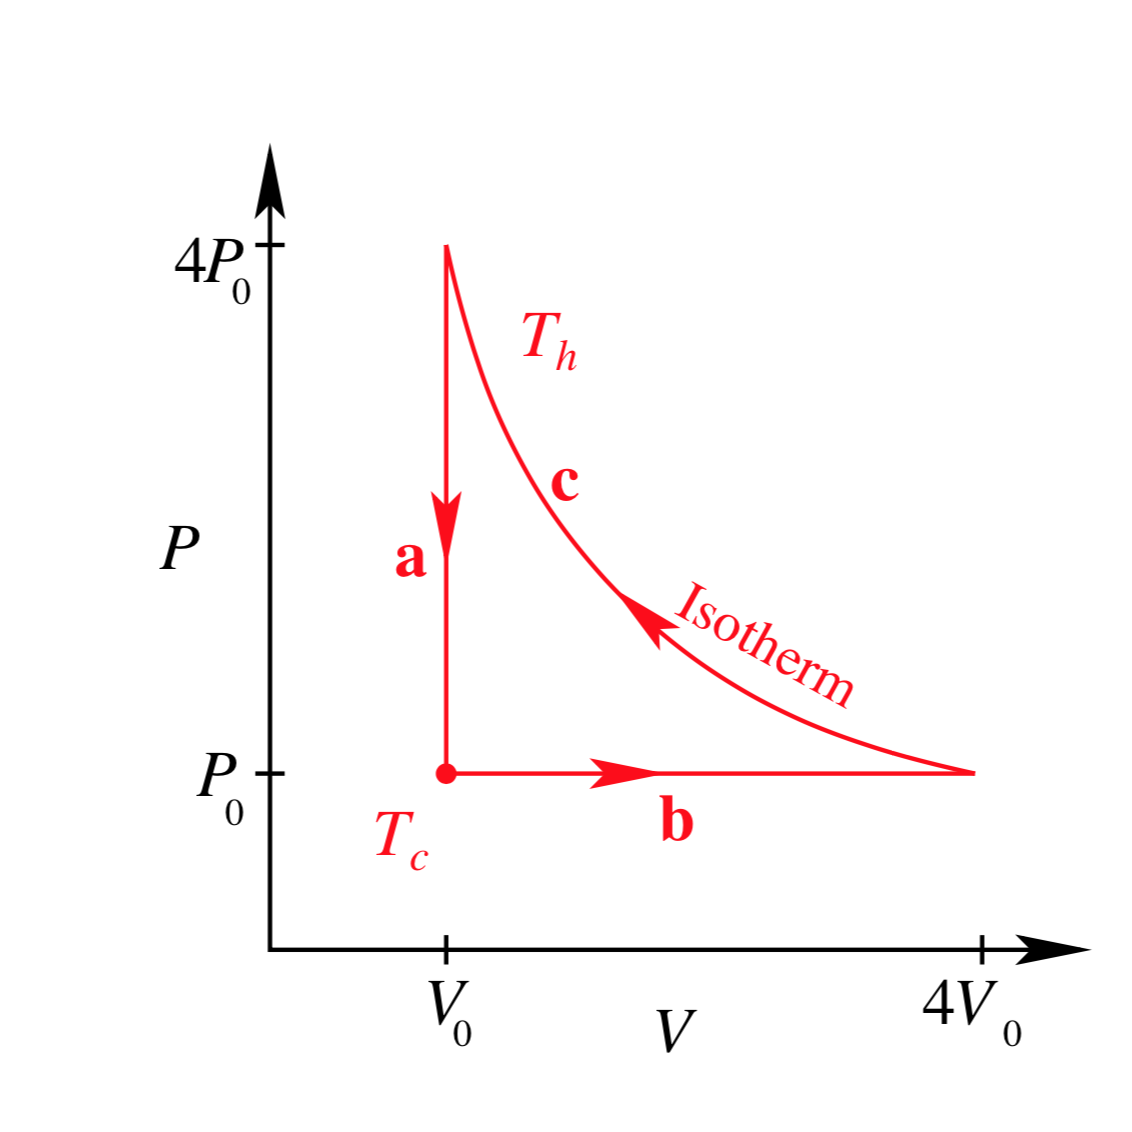
\includegraphics[width=0.3\linewidth]{PSet3_Fig1}
\caption{$P-V$ diagram.\label{P-V}}
\end{figure}

\begin{question}
Which of the following six statements are true?
\end{question}

\begin{enumerate}[(1)]
	\item The cycle is reversible; no net entropy is created in the Universe.
	\\
	\textbf{False.} Leg \textbf{a} and leg \textbf{b} both increase net entropy of the universe. The system is exchanging heat with a cold and hot bath, respectively, leading to an entropy increase of $\Delta S = \Delta Q/T$.

	\item The cycle acts as a refrigerator, using work from the piston to draw energy from the cold bath into the bot bath, cooling the bath.
	\\
	\textbf{False.} In leg \textbf{a}, when the system is in contact with the cold bath, heat energy is being transferred \textit{from} the system \textit{to} the cold bath.

	\item The cycle acts as an engine, transfering heat from the hot bath to the cold bath and doing positive net work on the outside world.
	\\
	\textbf{False.} $W = \int P \d{V} < 0$; the work done on the outside world is negative. Engines do positive work on their environments.

	\item The work done per cycle has magnitude
			$|W| = P_0V_0 |4\log{4-3}|$.
	\\
	\textbf{True.} It can be shown that the area integral $\int P \d{V}$ is equal to 	$P_0V_0 |4\log{4-3}|$ (i did it on the white board in discussion!).
	\item The heat transferred into the cold bath, $Q_c$, has magnitude	$|Q_c| = (9/2)P_0V_0$.
	\\
	\textbf{True.} Consider leg \textbf{a} (where no work is being done). The heat energy transferred is given by $Q = \Delta U - W$. Initially, the potential energy is $U_i = (3/2)NK_bT_h = (3/2)4P_0V_0$. Once the cycle reaching leg \textbf{b}, the potential energy is $U_f = (3/2)NK_bT_c = (3/2)P_0V_0$. Therefore, $Q = \Delta U = (9/2)P_0V_0$.

	\item The heat transferred from the hot bath, $Q_h$, plus the net work $W$ done by the piston onto the gas, equals the heat $Q_c$ transferred into the cold bath.
	\\
	\textbf{True.} This is a statement of total energy conservation in the system.
\end{enumerate}

\end{document}
